\chapter{Note sulla backpropagation}\label{ch-07}

Queste note contengono la \textbf{derivazione completa dell'algoritmo di
backpropagation}, l'algoritmo che risolve il problema del \emph{credit
assignment} nelle reti multistrato introdotto in
\href{06\%20-\%20Reti\%20neurali\%20(parte\%201)\%20-\%20dal\%20neurone\%20al\%20MLP}{06
- Reti neurali (parte 1) - dal neurone al MLP}. Il professore insiste su
un punto: \textbf{la derivazione va rifatta da sé, non memorizzata}.
Solo così si è in grado di ricalcolarla per loss, attivazioni o
architetture diverse --- ed è questo il vero obiettivo. Implementarla
nel progetto è il modo migliore per capirla a fondo.

Riferimenti: Rumelhart, Hinton, Williams, \emph{Parallel Distributed
Processing} (1986), cap. 8; Mitchell, \emph{Machine Learning}, cap. 4;
Haykin, \emph{Neural Networks}.

\section{Strumenti di calcolo
differenziale}\label{strumenti-di-calcolo-differenziale}

La discesa del gradiente richiede derivate di funzioni composte. Servono
tre regole: \[
\frac{\partial f}{\partial x} = \frac{\partial f}{\partial g}\cdot\frac{\partial g}{\partial x} \quad \text{(regola della catena)}, \qquad D[f(g(x))] = f'(g(x))\cdot g'(x), \qquad D[f\cdot g] = f'\cdot g + f\cdot g'.
\] La regola della catena è utile perché \textbf{scompone} il calcolo,
mettendo in evidenza ciò che si può calcolare immediatamente senza
perdere il filo generale.

\section{Il problema}\label{il-problema}

L'architettura di base è una rete feedforward completamente connessa
(MLP). Si usano indici diversi per gli strati: \(i\) per l'input, \(j\)
per lo strato nascosto, \(k\) per l'uscita.

\begin{figure}[htbp]
\centering
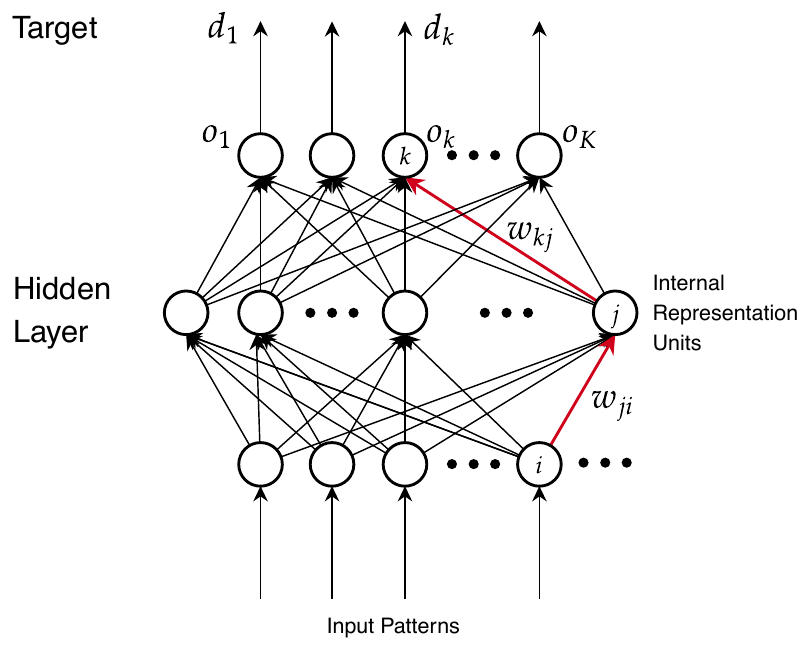
\includegraphics[width=0.54\linewidth,height=0.42\textheight,keepaspectratio]{images/07-bp_rete.png}
\caption{La rete di riferimento: input \(i\), unità nascoste \(j\), unità di
uscita \(k\).}
\end{figure}

\begin{boxdefinition}{Il problema della backpropagation}

Stimare il \textbf{contributo delle unità nascoste all'errore} in
uscita. Lo si fa calcolando la \textbf{regola delta generalizzata}
(\emph{Generalized Delta Rule}).

\end{boxdefinition}

Il training set è
\(TR = \{(\mathbf{x}^1, \mathbf{d}^1), \dots, (\mathbf{x}^l, \mathbf{d}^l)\}\)
(apprendimento supervisionato). Ogni unità di input \(i\) carica la
componente \(x_i\) del pattern: \(o_i = x_i\).

L'\textbf{errore totale} della rete sul training set è \[
E_{tot} = \sum_p E_p, \qquad E_p = \frac{1}{2}\sum_{k=1}^{K}(d_k - o_k)^2,
\] dove \(E_p\) è l'errore sul pattern \(p\) calcolato su tutte le \(K\)
unità di uscita. (Il fattore \(\frac{1}{2}\) serve solo a semplificare
la derivata.) Per alleggerire la notazione, d'ora in poi l'indice \(p\)
viene omesso: \(o_k\) sta per \(o_k(\mathbf{x}_p)\) e \(d_k\) per
\(d_{p,k}\).

\textbf{Obiettivo}: trovare i pesi \(\mathbf{w}\) che minimizzano
\(E_{tot}\) (per ora solo il termine sui dati). È ancora una
minimizzazione ai minimi quadrati (LMS). \textbf{Idea}: scendere lungo
la superficie di \(E_{tot}\) seguendo il gradiente.

\begin{figure}[htbp]
\centering
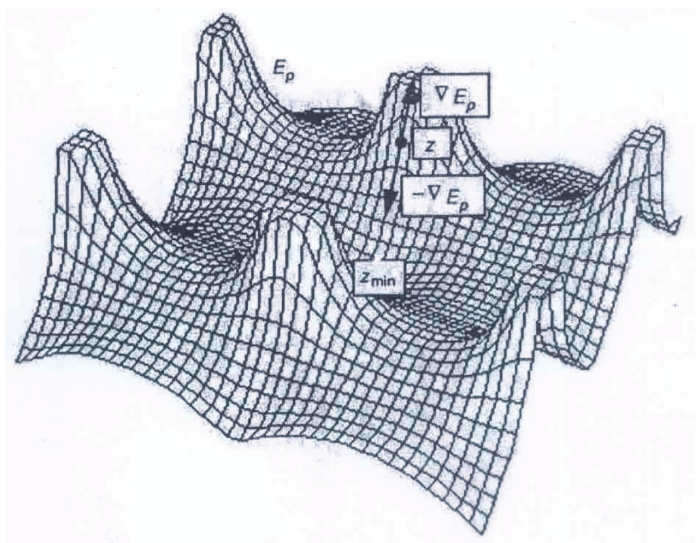
\includegraphics[width=0.54\linewidth,height=0.42\textheight,keepaspectratio]{images/07-bp_superficie.png}
\caption{Un paesaggio di \(E_{tot}\) nello spazio di due pesi: seguendo
\(-\nabla E\) dal punto \(Z\) si raggiunge \(Z_{min}\). A differenza del
modello lineare, la superficie non è convessa.}
\end{figure}

\section{L'algoritmo iterativo}\label{lalgoritmo-iterativo}

Si calcola la loss, se ne calcola il gradiente, si aggiornano tutti i
pesi; si ripete fino a convergenza o a un altro criterio di arresto.

\begin{boxabstract}{Algoritmo 1 --- Backpropagation}

Inizializzare tutti i pesi \(\mathbf{w}\) della rete e \(\eta\).
Calcolare le uscite delle unità ed \(E_{tot}\). \textbf{Finché}
\(E_{tot} > \epsilon\) (o altro criterio): - per ogni
\(w \in \mathbf{w}\):
\(\Delta w = -\dfrac{\partial E_{tot}}{\partial w}\) \textbf{(passo 1)};
- \(w_{new} = w + \eta\,\Delta w + \dots\) \textbf{(passo 2)}; -
ricalcolare le uscite ed \(E_{tot}\).

\end{boxabstract}

Esistono le versioni stocastica (on-line) e batch. Bisogna distinguere
due aspetti:

\begin{enumerate}
\def\labelenumi{\arabic{enumi}.}
\tightlist
\item
  il \textbf{calcolo del gradiente} \(\partial E_{tot}/\partial w\), per
  ogni peso della rete: è ciò che fa la backpropagation;
\item
  la \textbf{regola di aggiornamento} dei pesi: backprop standard,
  Quickprop, R-prop, \ldots{}
\end{enumerate}

Ci concentriamo sul passo 1: \[
\Delta w = -\frac{\partial E_{tot}}{\partial w} = -\sum_p \frac{\partial E_p}{\partial w} \overset{def}{=} \sum_p \Delta_p w.
\]

\section{La derivazione}\label{la-derivazione}

\subsection{Il gradiente per un peso
generico}\label{il-gradiente-per-un-peso-generico}

Consideriamo un peso generico \(w_{tu}\), che collega l'input
proveniente da un'unità generica \(u\) (che può essere \(i\) o \(j\))
all'unità generica \(t\). Poiché \[
net_t = \sum_s w_{ts}\,o_s, \qquad o_t = f_t(net_t),
\] applicando la regola della catena attraverso \(net_t\): \[
\Delta_p w_{tu} = -\frac{\partial E_p}{\partial w_{tu}} = \underbrace{-\frac{\partial E_p}{\partial net_t}}_{\delta_t}\cdot\underbrace{\frac{\partial net_t}{\partial w_{tu}}}_{o_u} = \delta_t\cdot o_u.
\] Infatti
\(\frac{\partial net_t}{\partial w_{tu}} = \frac{\partial \sum_s w_{ts} o_s}{\partial w_{tu}} = o_u\):
tutti i termini della somma sono costanti rispetto a \(w_{tu}\) tranne
quello con \(s = u\). (Gli \(o_s\) sono gli input dell'unità \(t\).)

Abbiamo definito il \textbf{delta dell'unità \(t\)}: \[
\delta_t = -\frac{\partial E_p}{\partial net_t}.
\] Espandiamolo ancora con la regola della catena, passando per
\(o_t = f_t(net_t)\): \[
\delta_t = -\frac{\partial E_p}{\partial net_t} = -\frac{\partial E_p}{\partial o_t}\cdot\frac{\partial o_t}{\partial net_t} = -\frac{\partial E_p}{\partial o_t}\cdot f'_t(net_t).
\] Resta da calcolare \(-\frac{\partial E_p}{\partial o_t}\), e qui si
distinguono due casi: \(t\) è un'\textbf{unità di uscita} \(k\), oppure
un'\textbf{unità nascosta} \(j\).

\subsection{\texorpdfstring{Caso 1: unità di uscita
(\(t = k\))}{Caso 1: unità di uscita (t = k)}}\label{caso-1-unituxe0-di-uscita-t-k}

L'uscita \(o_k\) compare direttamente in \(E_p\): \[
-\frac{\partial E_p}{\partial o_k} = -\frac{\partial\,\frac{1}{2}\sum_{r=1}^{K}(d_r - o_r)^2}{\partial o_k} = (d_k - o_k),
\] perché solo il termine \(r = k\) dipende da \(o_k\), e la sua
derivata è \(\frac{1}{2}\cdot 2(d_k - o_k)\cdot(-1)\). Quindi: \[
\boxed{\delta_k = (d_k - o_k)\cdot f'_k(net_k)}
\] È esattamente il delta già visto per la singola unità sigmoidale:
l'errore è direttamente misurabile perché conosciamo il target.

\subsection{\texorpdfstring{Caso 2: unità nascosta
(\(t = j\))}{Caso 2: unità nascosta (t = j)}}\label{caso-2-unituxe0-nascosta-t-j}

Per un'unità nascosta non c'è un target: \(o_j\) non compare
direttamente in \(E_p\). Però \(o_j\) influenza \(E_p\)
\textbf{attraverso tutte le unità di uscita} a cui è collegata: ogni
\(net_k\) dipende da \(o_j\). Applicando la regola della catena con una
somma su tutte le \(k\): \[
-\frac{\partial E_p}{\partial o_j} = \sum_{k=1}^{K}\underbrace{-\frac{\partial E_p}{\partial net_k}}_{\delta_k}\cdot\frac{\partial net_k}{\partial o_j} = \sum_{k=1}^{K}\delta_k\, w_{kj},
\] poiché
\(\frac{\partial net_k}{\partial o_j} = \frac{\partial \sum_s w_{ks}\,o_s}{\partial o_j} = w_{kj}\).
Quindi: \[
\boxed{\delta_j = \left(\sum_{k=1}^{K}\delta_k\, w_{kj}\right)\cdot f'_j(net_j)}
\]

\begin{boxtip}{Il punto cruciale}

Il termine \(-\frac{\partial E_p}{\partial net_k}\) \textbf{lo abbiamo
già calcolato}: è \(\delta_k\)! Il delta di un'unità nascosta si ottiene
quindi \textbf{propagando all'indietro} i delta delle unità di uscita,
pesati con gli stessi pesi \(w_{kj}\) usati nella propagazione in
avanti. Da qui il nome \textbf{back-propagation}: l'errore ``risale'' la
rete. Questo risolve il credit assignment: la ``colpa'' di un'unità
nascosta è la somma delle colpe delle unità a cui contribuisce, pesata
da quanto contribuisce.

\end{boxtip}

\begin{figure}[htbp]
\centering
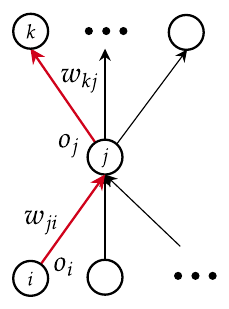
\includegraphics[width=0.21\linewidth,height=0.42\textheight,keepaspectratio]{images/07-bp_localita.png}
\caption{Usare il grafo della rete per localizzare il calcolo: ogni termine
coinvolge solo unità e pesi adiacenti.}
\end{figure}

Alcune osservazioni sul caso 2:

\begin{itemize}
\tightlist
\item
  esprime la variazione di \(E_p\) considerando \textbf{tutte} le unità
  di uscita \(o_k\);
\item
  ogni \(o_k\) (e \(net_k\)) dipende da \(o_j\): per questo compare la
  somma su \(k\);
\item
  lo stesso risultato si può ottenere direttamente dalla definizione di
  \(E_p\) (per esercizio), ma questa forma è più istruttiva perché
  mostra il flusso delle derivate parziali \textbf{sulla rete}.
\end{itemize}

\section{Sintesi delle formule}\label{sintesi-delle-formule}

Per due strati abbiamo derivato: \[
\Delta_p w_{tu} = \delta_t\cdot o_u,
\] dove \(\delta_t\) è il \textbf{segnale d'errore} disponibile
all'unità \(t\) e \(o_u\) è l'input a \(t\) proveniente da \(u\)
(attraverso la connessione \(w_{tu}\)). In particolare:

{\def\LTcaptype{none} % do not increment counter
\begin{longtable}[]{@{}
  >{\raggedright\arraybackslash}p{(\linewidth - 4\tabcolsep) * \real{0.3333}}
  >{\raggedright\arraybackslash}p{(\linewidth - 4\tabcolsep) * \real{0.3333}}
  >{\raggedright\arraybackslash}p{(\linewidth - 4\tabcolsep) * \real{0.3333}}@{}}
\toprule\noalign{}
\begin{minipage}[b]{\linewidth}\raggedright
Peso
\end{minipage} & \begin{minipage}[b]{\linewidth}\raggedright
Aggiornamento
\end{minipage} & \begin{minipage}[b]{\linewidth}\raggedright
Delta
\end{minipage} \\
\midrule\noalign{}
\endhead
\bottomrule\noalign{}
\endlastfoot
\(w_{kj}\) (nascosta → uscita) & \(\Delta_p w_{kj} = \delta_k\cdot o_j\)
& \(\delta_k = (d_k - o_k)\,f'_k(net_k)\) \\
\(w_{ji}\) (input → nascosta) & \(\Delta_p w_{ji} = \delta_j\cdot o_i\)
& \(\delta_j = \left(\sum_{k}\delta_k\,w_{kj}\right) f'_j(net_j)\) \\
\end{longtable}
}

\begin{figure}[htbp]
\centering
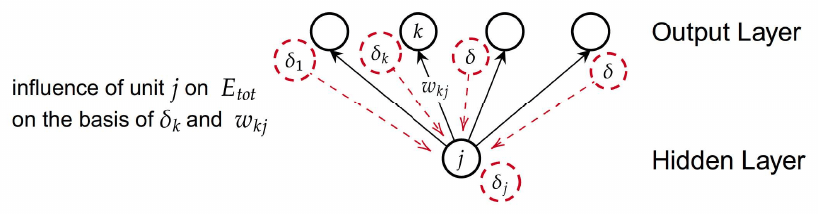
\includegraphics[width=0.71\linewidth,height=0.42\textheight,keepaspectratio]{images/07-bp_retropropagazione.png}
\caption{Retropropagazione dei delta: l'influenza dell'unità nascosta \(j\) su
\(E_{tot}\) si calcola dai \(\delta_k\) dello strato superiore e dai
pesi \(w_{kj}\).}
\end{figure}

\subsection{\texorpdfstring{Generalizzazione a \(m\) strati
nascosti}{Generalizzazione a m strati nascosti}}\label{generalizzazione-a-m-strati-nascosti}

La derivazione vale per \textbf{qualsiasi numero di strati nascosti}: i
delta non arrivano solo dallo strato di uscita, ma da qualsiasi strato
superiore \(h\) a cui l'unità è collegata. In generale, \textbf{i delta
arrivano da tutte le unità a cui l'unità corrente è connessa}: \[
\delta_j = \left(\sum_{h \in \text{successori}(j)}\delta_h\,w_{hj}\right) f'_j(net_j).
\] La regola di aggiornamento per ogni pattern (omettendo \(p\)) è \[
w_{tu}^{new} = w_{tu} + \eta\,\delta_t\,o_u.
\] Usando \(\Delta_p w\) per ogni pattern si ottiene la versione
\textbf{on-line}; per la versione \textbf{batch} si sommano i contributi
su tutti i pattern prima di aggiornare.

\section{Il ciclo di addestramento
completo}\label{il-ciclo-di-addestramento-completo}

\begin{enumerate}
\def\labelenumi{\arabic{enumi}.}
\tightlist
\item
  \textbf{Calcolo in avanti} (\emph{forward}): uscite di tutte le unità,
  strato per strato.
\item
  Calcolo degli \textbf{errori e dei delta nello strato di uscita}.
\item
  \textbf{Propagazione all'indietro} dei delta dallo strato di uscita
  agli strati nascosti.
\item
  \textbf{Aggiornamento dei pesi}.
\item
  Si ricomincia, fino al criterio di arresto.
\end{enumerate}

\begin{boxwarning}{Non dimenticare i bias}

Calcolo e aggiornamento vanno applicati anche ai \textbf{bias} di tutte
le unità: si assume la prima componente dell'input di ogni unità pari a
1, con il bias come peso \(w_{t0}\). Quindi
\(\Delta w_{t0} = \delta_t \cdot 1\).

\end{boxwarning}

\section{Proprietà e
interpretazione}\label{proprietuxe0-e-interpretazione}

\begin{itemize}
\tightlist
\item
  \textbf{Calcoli solo locali}: ogni unità usa direttamente solo
  informazioni vicine (le unità sotto e sopra), non strati lontani; il
  resto arriva indirettamente tramite il flusso dei delta. In altre
  parole: nonostante il calcolo sia locale, la modifica di un peso ha un
  \textbf{effetto globale} sulla rete. Qual è l'influenza di ciascun
  \(w_{tu}\) sull'errore globale? Questo effetto complesso è stato
  \textbf{scomposto} in componenti semplici tramite i delta locali a
  ogni unità.
\item
  \textbf{Visione come processo di diffusione}: la backpropagation è una
  propagazione locale spazio-temporale dai ``genitori'' dell'unità
  all'unità e dall'unità ai suoi ``figli''.
\item
  \textbf{Efficienza --- la ``fattorizzazione magica''}: il delta
  \(\delta_t\) di ogni unità si calcola \textbf{una sola volta} e si
  riusa per \textbf{tutti} i suoi pesi \(w_{tu}\). Il costo è quindi
  proporzionale al \textbf{numero di pesi}, non al suo quadrato. Con
  modelli da miliardi di pesi la differenza è enorme: \(10^9\) contro
  \((10^9)^2 = 10^{18}\) operazioni, che sarebbe infattibile.
\end{itemize}

\begin{boxtip}{Tre livelli di lettura della derivazione}

\begin{enumerate}
\def\labelenumi{\arabic{enumi}.}
\tightlist
\item
  I singoli \textbf{passaggi matematici}.
\item
  L'\textbf{interpretazione} delle variazioni locali di una quantità
  rispetto alle altre (il significato delle derivate parziali).
\item
  Il \textbf{quadro generale}: la scomposizione serve a trovare i valori
  delta di ogni livello, scomponendo l'errore \textbf{sulla rete} che si
  ha davanti.
\end{enumerate}

\end{boxtip}

\begin{boxwarning}{Terminologia corretta}

Non si dice ``rete backprop'': la rete neurale è il \textbf{modello}. La
backpropagation è un \textbf{algoritmo di addestramento} basato sulla
retropropagazione degli errori, cioè sul calcolo diretto del gradiente
attraverso la rete.

\end{boxwarning}

\begin{boxexample}{Esempio numerico (per verificare la comprensione)}

Rete con un input \(x = 1\), una unità nascosta sigmoidale e una di
uscita lineare, senza bias; pesi \(w_{ji} = 0{,}5\), \(w_{kj} = 1\),
target \(d = 1\), \(\eta = 0{,}1\). - Forward: \(net_j = 0{,}5\),
\(o_j = \sigma(0{,}5) \approx 0{,}622\);
\(o_k = 1 \cdot 0{,}622 = 0{,}622\). - Delta di uscita (lineare,
\(f' = 1\)): \(\delta_k = (1 - 0{,}622)\cdot 1 = 0{,}378\). - Delta
nascosto:
\(\delta_j = (\delta_k w_{kj})\,\sigma'(net_j) = 0{,}378 \cdot 0{,}622 \cdot (1 - 0{,}622) \approx 0{,}089\).
- Aggiornamenti:
\(\Delta w_{kj} = \eta\,\delta_k\,o_j \approx 0{,}1 \cdot 0{,}378 \cdot 0{,}622 \approx 0{,}0235\);
\(\Delta w_{ji} = \eta\,\delta_j\,x \approx 0{,}0089\).

Entrambi i pesi aumentano, facendo crescere l'uscita verso il target.

\end{boxexample}

\begin{boxquestion}{Possibili domande d'esame}

\begin{itemize}
\tightlist
\item
  Derivare la backpropagation per un MLP a due strati con errore
  quadratico.
\item
  Cos'è \(\delta_t\)? Come si calcola per un'unità di uscita e per
  un'unità nascosta?
\item
  Perché la backpropagation ha costo lineare nel numero dei pesi?
\item
  Come cambia la derivazione con una loss diversa o con più strati
  nascosti?
\end{itemize}

\end{boxquestion}
